\subsection{Двойственный по Пуанкаре к замкнутому подмногообразию}

	Пусть $M$~--- ориентированное многообразие размерности $n$, а $S \subset M$~--- замкнутое ориентированное подмногообразтие\footnote{Тут слово "замкнутое" имеет смысл "замкнутое подмножество"; $S$ далеко не обязано быть компактным. } размерности $k$.

	Пусть  $i\colon S \hookrightarrow M$~--- вложение, тогда $S$ мы можем однозначно сопоставить некоторый класс $[\eta_{S}] \in H^{n - k}(M)$ следующим образом. 

	Пусть $\omega$~--- замкнутая $k$-форма на $M$ с компактным носителем. Так как $S$ замкнутое, $\supp(\omega\vert_{S}) \subset S \cap \supp(\omega)$ компактно в $M$ как замкнутое подмножество компакта. Тогда корректно определён интеграл $\int_{S} i^* \omega$, так как форма $i^* \omega$ имеет компактный носитель в $S$, $i^* \omega \in \Omega_{c}^k(S)$. 

	Соответственно, тогда $\int\limits_{S}$ индуцирует линейный функционал на $H_{c}^k(M)$. Тогда, так как по двойственности Пуанкаре $(H_c^{k})^* \cong H^{n - k}(M)$, интегрированию по $S$ однозначно соответствует некоторый класс $[\eta_S] \in H^{n - k}(M)$. Более того, как мы помним из конструкции
	\[
		\int\limits_{S} i^* \omega = \int\limits_{M} \omega \wedge \eta_S \quad \forall [\omega] \in H^k_{c}(M).
	\]
	И, как мы помним, это эквивалентное определение. То есть, если мы хотим проверить, что класс какой-то формы является двойственным по Пуанкаре к компактному подмногообразию $S$, нужно проверять именно это условие. 

	Этот класс мы и будем называть \bf{(замкнутым) двойственным по Пуанкаре классом к $S$}. 


	Теперь пусть $S$~--- компактное подмногообразие. В этом случае можно сделать всё то же самое (и, двойственный по Пуанкаре существует), но ситуация несколько улучшается. 

	В этом случае у $S$ есть еще и \bf{компактный двойственный по Пуанкаре}. Действительно, $\int\limits_{S}$ определяет линейный функционал на $H^k(M)$ (вот тут мы пользуемся компактностью $M$), а тогда по двойственности Пуанкаре 
	\[
		\exists ! \quad [\eta_S'] \in H_c^{n - k}(M).
	\]

	Тут мы предполагаем, что $M$ обладает конечным хорошим покрытием, чтоб выполнялся изоморфизм 
	\[
		(H^k(M))^* \cong H_c^{n - k}(M).
	\]

	Компактный двойственный по Пуанкаре класс характеризуется таким свойством: 
	\[
		\int\limits_{S} i^* \omega = \int\limits_{M} \omega \wedge \eta'_S \quad \forall \omega \in H^k(M).
 	\]

 	Отсюда видно, что в частности компактный двойственный по Пуанкаре является и замкнутым двойственным по Пуанкаре (как форма). Но отметим тут также, что сами классы в когомологиях могут быть совсем разными (и в задачах у нас есть такие примеры). 


 	\begin{example}
 	 	\textcolor{red}{Дописать сюда вычисления примеров и разгон про замкнутые гомологии и компактные гомологии}.
 	 \end{example} 

 	 Пусть теперь мы работаем с компактным случаем, а  $W \subset M$~--- открытое подмножество, содержащее $S$. Тогда компактный двойственный по Пуанкаре к $S$ в многообразии $W$ (назовём его $\eta'_{S, W} \in H_c^{n - k}(W)$) продолжается нулём до компактного двойственного по Пуанкаре к $S$ в $M$ (его назовём $\eta_{S}' \in H_c^{n - k}(M)$):
 	 \[
 	 	\int_{S} i^* \omega = \int\limits_{W} \omega \wedge \eta'_{S, W} = \int\limits_{M} \omega \wedge \eta'_{S}.
 	 \]

 	 Отсюда следует, что носитель компактного двойственного по Пуанкаре может быть стянут до любой окрестности $S$! И эту окрестность мы можем выбирать.  



 	 \subsection{Напоминание про векторные расслоения и класс Тома}


 	 \begin{definition} 
 	 	Пусть $\pi\colon E \to M$~--- сюръективное отображений многообразий, причём $\forall x \in M \ \pi^{-1}(x)$~--- векторное пространство. 

 	 	Тогда $(E, \pi)$ называется \emph{гладким вещественным векторным расслоением} ранга $n$, если существует открытое покрытие $M$ множествами $\{ U_{\alpha} \}$  и набор отображений $\{ \varphi_{\alpha} \}_{\alpha} $ такой что 
 	 	\begin{itemize}
 	 		\item $\varphi_{\alpha}\colon \pi^{-1}(U_{\alpha}) \cong U_{\alpha} \times \R^n$~--- диффеоморфизм. 
 	 		\item $\forall x \in U_{\alpha}$ оторбражение $v \mapsto \varphi_{\alpha}^{-1}(x, v)$~--- это линейный изоморфизм между $\R^n$ и  $\pi^{-1}(x)$. Говоря короче, на каждом слое отображения $\varphi_{\alpha}$ являются линейными изоморфизмами. 

 	 		\item Отображения 
 	 		\[
 	 			\varphi_{\alpha} \circ \varphi_{\beta}^{-1}\colon (U_{\alpha} \cap U_{\beta}) \times \R^n \to (U_{\alpha} \cap U_{\beta}) \times \R^n
 	 		\]
 	 		на каждом слое являются автоморфизмами $\R^n$ и таким образом порождают отображения 
 	 		\[
 	 			g_{\alpha \beta}\colon U_{\alpha} \cap U_{\beta} \to \GL_{n}(\R), \quad g_{\alpha \beta} = \varphi_{\alpha} \circ \varphi_{\beta}^{-1}\vert_{\{ x \} \times \R^n}.
 	 		\]
 	 	\end{itemize}

 	 	\end{definition}

 	 	Далее все расслоения мы будем полагать именно такими. Кроме того, мы будем полагать, что многообразие $M$ ориентированно, переходы имеют положительный определитель и как следствие, расслоение $E$ также ориентированно (это нам понадобится, чтоб использовать формулу Стокса). 

 	 	\begin{remark}
 	 		Функции перехода $g_{\alpha \beta}$ удовлетворяют следующему условию: 
 	 	\[
 	 		g_{\alpha \beta} \circ g_{\beta \gamma} = g_{\alpha \gamma} \text{ на } U_{\alpha} \cap U_{\beta} \cap U_{\gamma}.
 	 	\]

 	 	Вообще говоря, если у нас есть покрытие $U_{\alpha}$ многообразия и набор гладких отображений перехода $g_{\alpha \beta}\colon U_{\alpha} \cap U_{\beta} \to \GL_n(\R)$, удовлетворяющих условию 
 	 	\[
 	 		g_{\alpha \beta} \circ g_{\beta \gamma} = g_{\alpha \gamma} \text{ на } U_{\alpha} \cap U_{\beta} \cap U_{\gamma},
 	 	\]
 	 	то при помощи этого набора данных мы можем построить векторное расслоение так: 
 	 	\[
 	 		\pi\colon U_{\alpha} \mapsto U_{\alpha} \times \R^n.
 	 	\]
 	 	\end{remark}

 	 	\begin{definition} 
 	 		Пусть $\pi\colon E \to M$~--- векторное расслоение. Определим $H^{\bullet}_{cv}(E)$~--- \emph{когомологии с компактным носителем в вертикальном направлении}. 

 	 		Мы будем рассматривать комплекс форм $\Omega^{\bullet}_{cv}(E)$~--- комплекс форм с компактным носителем \emph{в вертикальном направлении}. Это означает, что для $\omega \in \Omega^{\bullet}_{cv}(E)$ $\forall x \ \omega\vert_{\pi^{-1}(x)}$ имеет компактный носитель.  

 	 		Теперь заметим, что если $\omega \in \Omega^{\bullet}_{cv}(E)$, то $\mathrm{d} \omega \in \Omega^{\bullet}_{cv}(E)$ (так как дифференциал коммутирует с сужением на слой). Значит, $\Omega^{\bullet}_{cv}(E)$~--- дифференциальный комплекс. Его когомологии мы и будем называть когомологиями с компактным носителем в вертикальном направлении. 

 	 	\end{definition}

 	 	Определим отображение \emph{интегрирования вдоль слоя} следующим образом: 
 	 	\[
 	 		\pi_*\colon \Omega_{cv}^{\bullet}(E) \to \Omega^{\bullet - n}(M)	
 	 	\]

 	 	Рассмотрим сначала простой случай тривиального расслоения: $E = M \times \R^n$ и пусть $t_1, \ldots, t_n$~--- координаты в слое $\R^n$. Определим отображение отдельно на двух типах форм: 
 	 	\begin{itemize}
 	 		\item $\pi^*(\varphi) \wedge f(x, t_1, \ldots, t_m) \mathrm{d}t_{i_1} \wedge \ldots \mathrm{d}t_{i_r} \mapsto 0,$ если $r < n$. Иными словами, если в форме есть не все $\mathrm{d}t_j$, мы отправляем её в 0.

 	 		\item $\pi^*(\varphi) \wedge f(x, t_1, \ldots, t_n) \mathrm{d}t_1 \wedge \ldots \wedge \mathrm{d}t_n \mapsto \varphi \int\limits_{\pi^{-1}(x)} f(x, t_1, \ldots, t_n)$,
 	 	\end{itemize}
 	 	где $f$ имеет компактный носитель для любого фиксированного $ x \in M$ (так как у формы из $\Omega^{\bullet}_{cv}$ компактный носитель вдоль любого вертикального слоя), $\varphi \in \Omega^{\bullet}(M)$. 

 	 	В случае произвольного ориентированного расслоения мы будем определять отображение таким образом в тривиализациях, а после склеим (легко показать, что это не зависит от выбора тривиализации и согласовано на пересечениях, откуда мы получаем в итоге глобальную форму после склейки). 
 	 	
 	 	\begin{theorem} 
 	 		Интегрирование вдоль слоя коммутирует с внешним дифференцированием, то есть $\pi_* \mathrm{d} = \mathrm{d}\pi_*$.
 	 	\end{theorem}
 	 	\begin{proof}
 	 		Сначала посмотрим на формы второго типа. Там есть полный набор $\mathrm{d}t_j$, поэтому, когда мы продифференцируем, добавится лишь $x_j$ (а так как интегрируем мы по $\mathrm{d}t_j$, не важно, в каком порядке делать операции). 

 	 		Теперь посмотрим на формы первого типа. Из определения интегрирования вдоль слоёв: $\mathrm{d} \pi_* \omega = 0$. Чтоб показать, что $\pi_* \mathrm{d}\omega = 0$, разберём два случая: 
 	 		\begin{itemize}
 	 			\item Если у нас в форме $\mathrm{d}t_{i_1} \wedge \ldots \wedge \mathrm{d}t_{i_{r}}$ и $r < n - 1$, то после того, как мы продифференцируем, во всех слагаемых набор $\mathrm{d}t_j$ снова будет неполным и $\pi_*$ отправит форму в 0. 

 	 			\item Если $r = n - 1$, то когда заметим, что после дифференцирования мы будем применять $\pi_*$ к 
 	 			\[
 	 				(\pi^*\varphi) \frac{\partial \varphi}{\partial t_j}(x, t) \mathrm{d}t_j \wedge \mathrm{d}t_{i_1} \wedge \ldots \wedge \mathrm{d}t_{i_{r}}
 	 			\] 
 	 			а после того, как мы проинтегрируем по слою, каждое слагаемое будет содержать множитель
 	 			\[
 	 				\int\limits_{\R^{n}}  \frac{\partial f(x, t)}{\partial t_j} \mathrm{d}t_j \wedge \mathrm{d}t_{i_1} \wedge \ldots \wedge \mathrm{d}t_{i_{r}} = \int\limits_{\R^{n - 1}} \lr*{\ \int\limits_{-\infty}^{+\infty} f(x, t) \mathrm{d} t_j} \mathrm{d}t_{i_1} \wedge \ldots \wedge \mathrm{d}t_{i_{r}},
 	 			\]
 	 			а так как $f(x, t)$ имеет компактный носитель при фиксированном $x$, мы получаем 
 	 			\[
 	 				\int\limits_{-\infty}^{+\infty} f(x, t) \mathrm{d} t_j = f(\ldots, + \infty, \ldots) - f(\ldots, -\infty, \ldots) = 0,	
 	 			\]
 	 			откуда видно, что вся сумма равна нулю. 
 	 		\end{itemize}
 	 	\end{proof}

 	 	\begin{theorem}[Формула проекции] 
 	 		Пусть $\pi\colon E \to M$~--- ориентированное векторное рассслоение ранга $n$, а $\tau$~--- форма на $M$ и $\omega \in \Omega_{cv}^{\bullet}(E)$. Тогда 
 	 		\[
 	 			\pi_*(\pi^*(\tau) \wedge \omega) = \tau \wedge \pi_* \omega. 
 	 		\]
 	 		Кроме того, если $M$ имеет размерность $m$, $\Omega_{cv}^{q}(E)$, $\tau \in \Omega_{c}^{m + n - q}(M)$, то 
 	 		\[
 	 			\int\limits_{E} (\pi^* \tau) \wedge \omega = \int\limits_{M} \tau \wedge \pi_* \omega. 
 	 		\]
 	 	\end{theorem}

 	 	Первое утверждение, как и обычно, технически проверяется для двух типов форм. Второе же утверждение можно (переходя к разбиению единицы) рассматривать локально, а локально это просто теорема Фубини. 


 	 	Доказательство леммы Пуанкаре для компактных носителей проводится дословно (пользуясь тем, что мы доказали выше) и даёт следующую лемму

 	 	\begin{lemma}[Лемма Пуанкаре для компактных вертикальных носителей] 
 	 		Интегрирование вдоль слоя задаёт изоморфизм 
 	 		\[
 	 			\pi_*\colon H^{\bullet}_{cv}(M \times \R^n) \to H^{\bullet - n}(M).
 	 		\]
 	 	\end{lemma}

 	 	А на самом деле, это частный случай следующего весьма общего утверждения: 

 	 	\begin{theorem}[Изоморфизм Тома] 
 	 		Пусть $M$~--- ориентированное многообразие, допускающее конечное хорошее покрытие, а $\pi\colon E \to M$~--- ориентированное векторное расслоение. Тогда 
 	 		\[
 	 			H^{\bullet}_{cv}(E) \cong H^{\bullet - n}(M).
 	 		\]
 	 	\end{theorem}
 	 	\begin{proof}
 	 		Как и обычно, используем принцип Майера-Виеториса. У нас есть точная последовательность комплексов
 	 		\begin{center}	
 	 			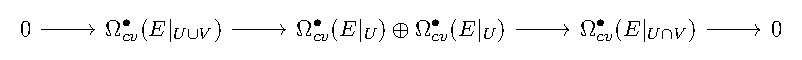
\includegraphics{lectures/7/pictures/cd_27.pdf}
 	 		\end{center}
 	 		Тогда интегрирование вдоль вертикальных слоёв индуцирует вот такую диаграмму:
 	 		\begin{center}
 	 			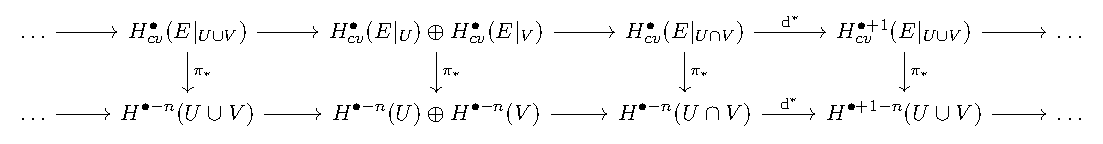
\includegraphics{lectures/7/pictures/cd_28.pdf}
 	 		\end{center}

 	 		Вообще говоря, нужно проверять, что она коммутативна. Для первых двух квадратов это очевидно (так там у нас вылазают формы на $M$, а их мы вдоль слоя не интегрируем, так что порядок не важен), проверим для третьего. Это следует из того, как устроен кограничный оператор и формулы проекции 
 	 		\[
 	 			\pi_* \mathrm{d}^* \omega = \pi_*((\pi^* \mathrm{d}\rho_U) \wedge \omega) = \lr*{\mathrm{d}\rho_U } \wedge \pi_* \omega = \mathrm{d}^* \pi_* \omega. 
 	 		\]

 	 		Если $U$ диффеоморфно $\R^n$, то утверждение сводится к лемме Пуанкаре для когомологий с компактным вертикальным носителем. Из 5-леммы мы знаем, что если утверждение верно для $U$,  $V$, $U \cap V$, то оно верно для $U \cup V$. 

 	 		Далее доказательство проводится индукцией по размеру хорошего покрытия (как и обычно). 
 	 	\end{proof}

 	 	Соответственно, рассмотрим изоморфизм Тома, но в другую сторону: 
 	 	\[
 	 		\cT\colon H^{\bullet}(M) \to H^{\bullet + n}(E). 
 	 	\]

 	 	\emph{Класс Тома} $\Phi \in H_{cv}^{\bullet + n}(E) $~--- образ класса $1 \in H^{0}(M)$, то есть $\cT(1)$. Легко видеть, что $\pi_* \Phi = \pi_* \cT(1) = 1$, откуда 
 	 	\[
 	 		\pi_*(\pi^*\omega \wedge \Phi) = \omega \wedge \pi_*\Phi = \omega. 
 	 	\]

 	 	 Отсюда видно, что изоморфизм тома $\cT$ (обратный к интегрированию вдоль вертикальных слоёв) задаётся формулой 
 	 	 \[
 	 	 	\cT(\omega) = \pi^*(\omega) \wedge \Phi,
 	 	 \]
 	 	 так как формула выше означает, что $\pi_* \cT = \id$. 

 	 	 Заметим также, что сужение класса тома $\Phi \in H^q_{cv}(E)$ на каждый слой $F$ даёт нам образующую $H^q_{c}(F)$, так как $\pi_* \Phi = 1$, что и означает, что 

 	 	 \[
 	 	 	\int\limits_{\R^n} \Phi = 1.
 	 	 \]

 	 	 \noindent\bf{Связь двойственности Пуанкаре и класса Тома.}

 	 	 Пусть $S$~--- замкнутое ориентированное подмногообразие размерности $k$ в $n$. Напомним, что двойственный по Пуанкаре к $S$ класс когомологий $[\eta_S] \in H^{n - k}(M)$ определяется условием 
 	 	 \[
 	 	 	\int\limits_{S} i^* \omega = \int\limits_{M} \omega \wedge \eta_S \quad \forall \omega \in H^k(M).
 	 	 \]


 	 	 Пусть $W$~--- трубчатая окрестность $S$ в $M$. Напомним, что она диффеоморфна \emph{нормальному расслоению}~--- такому векторному $\nu_S$ расслоению ранга $n - k$ над $S$, что последовательность расслоений
 	 	 \[
 	 	 	0 \to TS \to TM\vert_{S} \to \nu_S \to 0
 	 	 \]
 	 	 точна . Как мы помним, это расслоение ориентированно так, что расслоение 
 	 	 \[
 	 	 	\nu_S \oplus TS = TM\vert_{S}
 	 	 \]
 	 	 имеет ориентацию прямой суммы. 

 	 	 Применим изоморфизм Тома к нормальному расслоению/трубчатой окрестности $W \cong \nu_S$ над $S$:

 	 	 \begin{center}
 	 	 	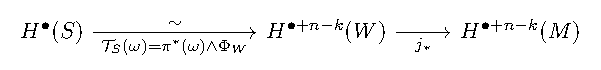
\includegraphics{lectures/7/pictures/cd_29.pdf}
 	 	 \end{center}

 	 	 где $\Phi_{W}$~--- класс Тома трубчатой окрестности, а $j_*$~--- его продолжение нулём на $M$ (тут всё корректно, так как из-за того, что у него компактный носитель вдоль верткиальных слоёв, он нулевой в окрестности границы $W$). 

 	 	 \begin{statement} 
 	 	 	$\eta_{S} = j_* \Phi \in H^{n - k}(M)$.
 	 	 \end{statement}

 	 	 \begin{proof}
 	 	 	Нам надо проверить, что 
 	 	 	\[
 	 	 		\forall \omega \in H_c^k(M) \quad \int\limits_{S} i^* \omega = \int\limits_{M} \omega \wedge \eta_{S}.
 	 	 	\]
 	 	 	Пусть $\pi\colon W \to S$~--- проекция, а $i$~--- вложение $S \hookrightarrow W$ в качестве нулевого сечения. Как мы помним, $\pi$ деформационно ретрагирует $W$ на $S$, откуда $\pi^*$ и $i^*$~--- изоморфизы на когомологиях. Тогда формы $\omega $ и $\pi^* i^* \omega$ отличаются на точную форму, так как представляют один когомологический класс: 
 	 	 	\[
 	 	 		\omega = \pi^* i^* \omega + \mathrm{d}\alpha.
 	 	 	\]

 	 	 	Осталось написать некоторые вычисления: 
 	 	 	\[
 	 	 		\int\limits_{M} \omega \wedge j_* \Phi = \int\limits_{W} \omega \wedge \Phi = \int\limits_{W} (\pi^* i^* \omega + \mathrm{d}\alpha) \wedge \Phi =
 	 	 	\]
 	 	 	теперь применим формулу Стокса (которая убьет лишнее слагаемое) и после формулу проекции: 
 	 	 	\[
 	 	 		= \int\limits_{W} \pi^* i^* \omega \wedge \Phi  = \int\limits_{S} i^* \omega \wedge \pi_* \Phi = \int\limits_{S} i^* \omega,
 	 	 	\]
 	 	 	так как $\pi_* \Phi = 1$.
 	 	 \end{proof}

 	 	 





 	 	
 	 

 	 


 	

